\documentclass[t]{beamer}
\usepackage[portuguese]{babel}
\usepackage[utf8]{inputenc}
\usetheme{Berkeley}
\usecolortheme{seahorse}

\addto\captionsportuguese{
	\renewcommand{\figurename}{Fig.}
	\renewcommand{\tablename}{Tab.}
}

\title{Tratamento de dados}
\subtitle{Como podemos tratar os dados dos dispositivos.}

\AtBeginSection[]
{
	\begin{frame}
	\frametitle{Sumário}
	\tableofcontents[currentsection]
\end{frame}
}

\begin{document}

\frame{\titlepage}

\begin{frame}
\frametitle{Sumário}
\tableofcontents
\end{frame}

\section{Tratamentos}

\begin{frame}{Tratamentos de dados}
Tipos de tratamento
\begin{itemize}
	\item Filtros
	\item Aprendizado
	\item Validação
\end{itemize}
\end{frame}

\begin{frame}{Porque tratar os dados?}
Big Data Vs:
\begin{itemize}
	\item Volume
	\item Velocidade
	\item Variedade
	\item Variabilidade
	\item Veracidade
	\item Validade
	\item Vulnerabilidade
	\item Volatilidade
	\item Visualização
	\item Valor
\end{itemize}
\end{frame}

\section{Filtros}
\begin{frame}{Filtros}
Tipos de filtros
\begin{itemize}
	\item Analógicos
	\item Digitais
	\item Contextuais
\end{itemize}
\end{frame}

\begin{frame}{Filtros}
Filtros comuns
\begin{itemize}
	\item Passa-alta (High Pass Filter)
	\item Passa-baixa (Low Pass Filter)
	\item Passa-banda (Band Pass Filter)
\end{itemize}
\end{frame}

\begin{frame}{Fusão de sensores}
Utilidades
\begin{itemize}
	\item Remover ruídos
	\item Decisões mais inteligentes
	\item Inferir informações
\end{itemize}
\end{frame}

\begin{frame}{Fusão de sensores}
Duplicação de sinal
\begin{figure}
	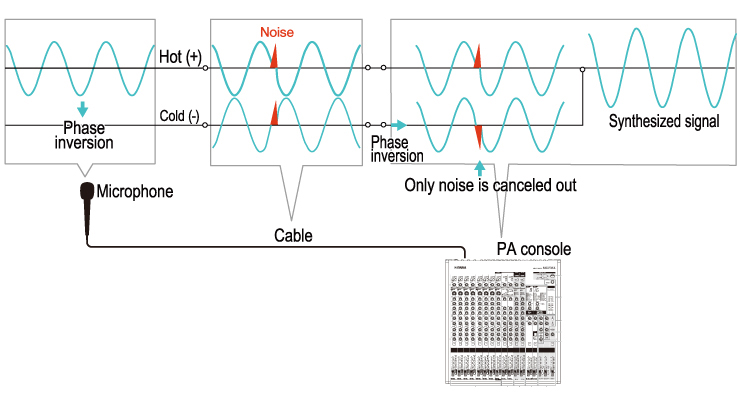
\includegraphics[width=\linewidth]{pa_beginners_cable_ph09}
\end{figure}
\end{frame}

\begin{frame}{Fusão de sensores}
Sensores magnéticos
\begin{figure}
	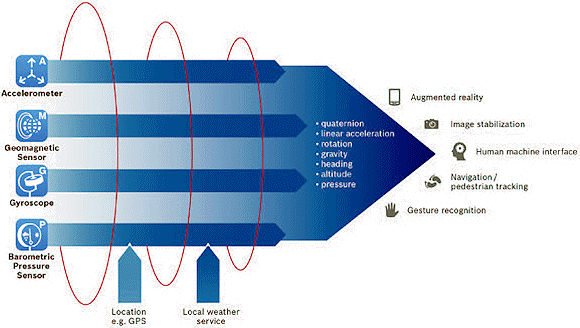
\includegraphics[width=\linewidth]{sensorfusion}
\end{figure}
\end{frame}

\begin{frame}{Fusão de sensores}
Exemplo com radares
\begin{figure}
	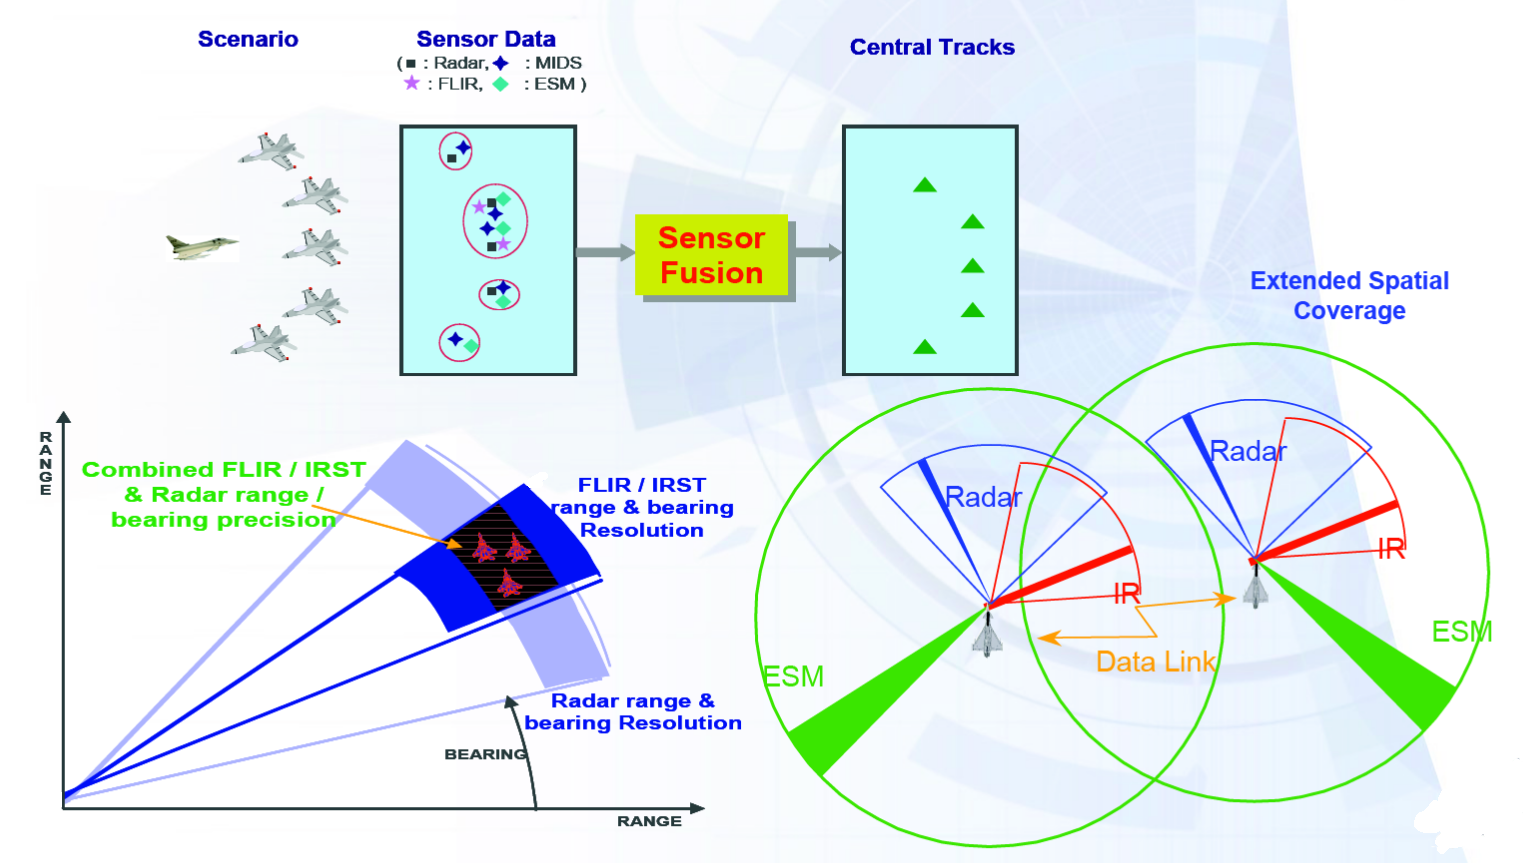
\includegraphics[width=\linewidth]{Eurofighter_sensor_fusion}
\end{figure}
\end{frame}

\begin{frame}{Fusão de sensores}
Carro autônomo
\begin{figure}
	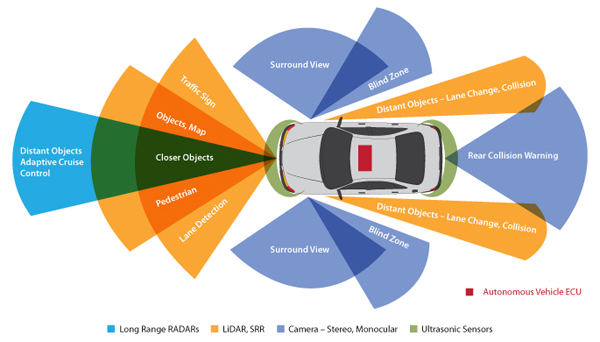
\includegraphics[width=\linewidth]{5_TataElxsiAutonomaisensorfusionschematic}
\end{figure}
\end{frame}

\begin{frame}{Fusão de sensores}
Carro autônomo
\begin{figure}
	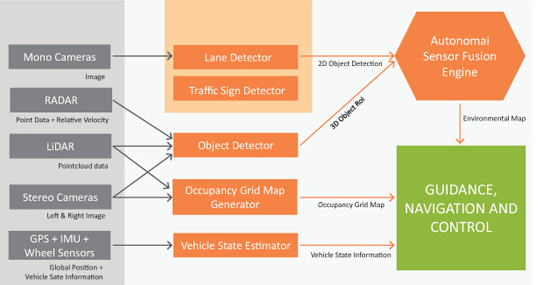
\includegraphics[width=\linewidth]{5_TataElxsiAutonomaiperceptionschematic}
\end{figure}
\end{frame}

\section{Aprendizado de Máquina}


\begin{frame}{Aprendizado de máquina}
Por que?!
\begin{itemize}
	\item Muitos dados
	\item Segurança para informações e sistemas
	\item Aumentar poder computacional
	\item Consumo eficiente de recursos e energia
	\item Crescimento constante de algoritmos e teorias
\end{itemize}
\end{frame}

\begin{frame}{Aprendizado de máquina}
\begin{figure}
	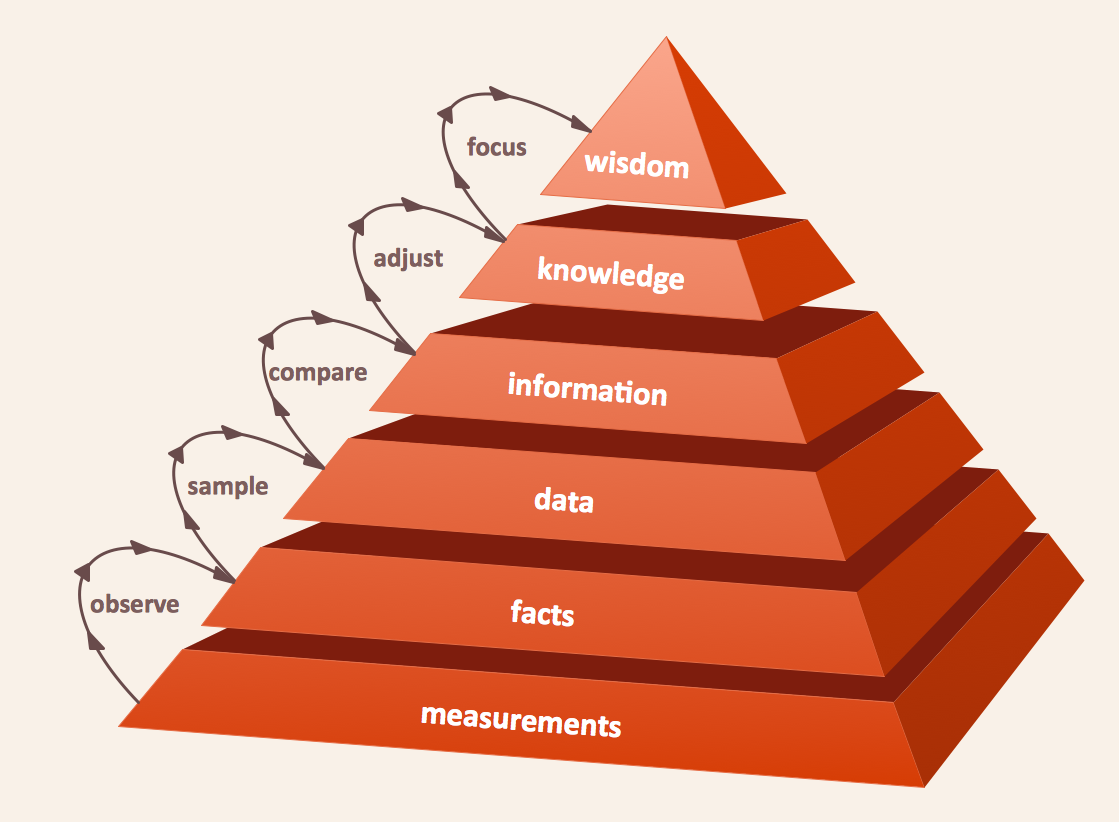
\includegraphics[width=\linewidth]{PYRAMID-DIKW-hierarchy-3d-pyramid}
\end{figure}
\end{frame}

\begin{frame}{Aprendizado de máquina}
\begin{figure}
	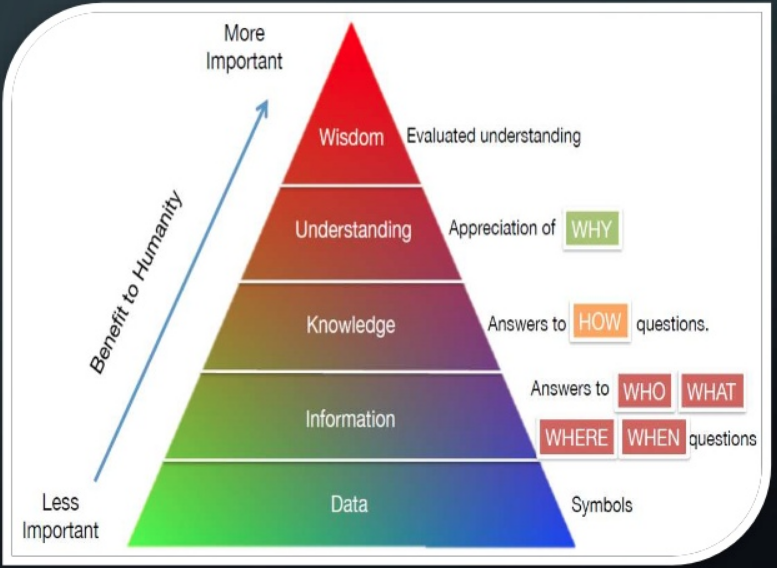
\includegraphics[width=\linewidth]{beneficiosdaanalisedosdados}
\end{figure}
\end{frame}

\begin{frame}{Aprendizado de máquina}
\begin{figure}
	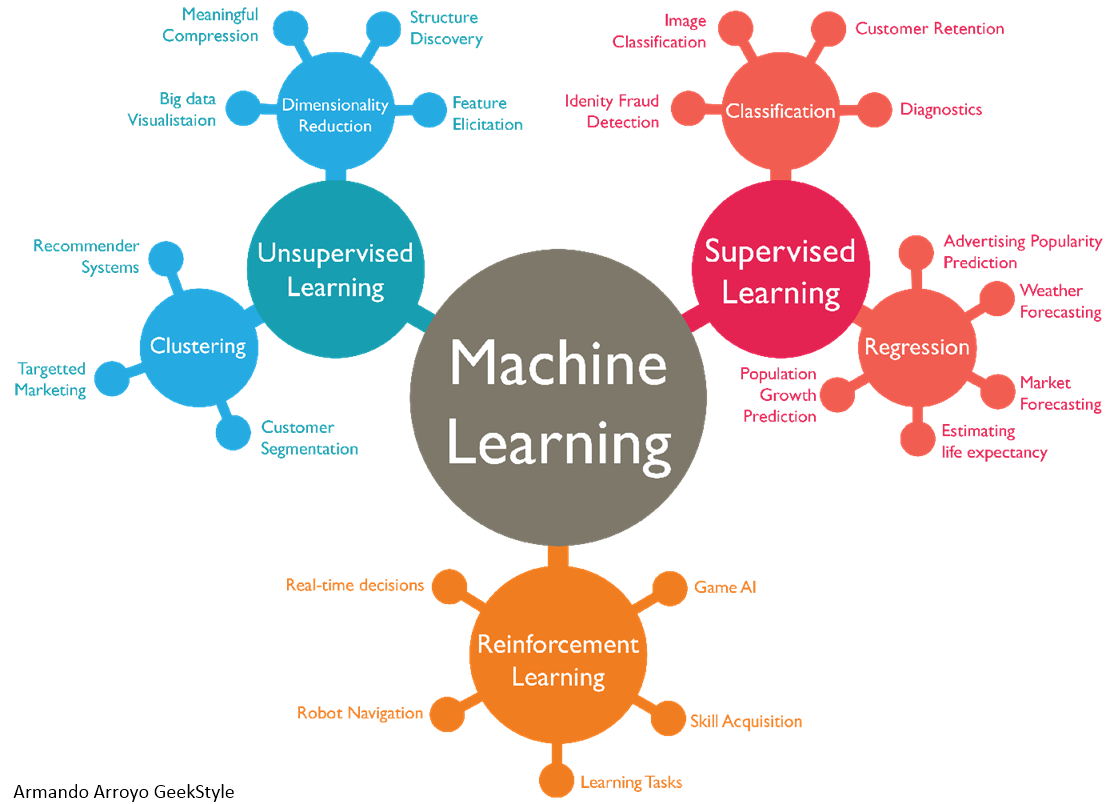
\includegraphics[width=\linewidth]{machinelearning}
\end{figure}
\end{frame}

\begin{frame}{Aprendizado de máquina}
Algoritmos
\begin{itemize}
	\item Classificação
	\begin{itemize}
		\item K-Nearest Neighbors~(KNN), Naive Bayes, Support Vector Machine~(SVM)
	\end{itemize}
	\item Regressão
	\begin{itemize}
		\item Linear Regression, Support Vector Regression, Random Forests, Bagging
	\end{itemize}
	\item Clusterização
	\begin{itemize}
		\item K-Means, Density-Based Spatial Clustering of Applications with Noise
	\end{itemize}
	\item Extração de características
	\begin{itemize}
		\item Principal Component Analysis~(PCA), Canonical Correlation Analysis, Feed Forward Neural Network
	\end{itemize}
	\item Detecção de anomalias
	\begin{itemize}
		\item One-class Support Vector Machines
	\end{itemize}
\end{itemize}
\end{frame}

\begin{frame}{Algoritmos}
K-Nearest Neighbors~(KNN)
\begin{itemize}
	\item Utilizado para classificar um novo dado desconhecido
	\item Utiliza um conjunto de dados de treinamento
	\item Para encontrar os vizinhos mais próximos utiliza:
	\begin{itemize}
		\item Euclidean distance
		\item $L_\infty$ norm
		\item Ângulo
		\item Mahalanobis distance
		\item Hamming distance
	\end{itemize}
	\item Requer armazenar o conjunto de dados de treinamento
	\item Exemplo de uso:
	\begin{itemize}
		\item Classificação de regularidades em padrão de navegação
	\end{itemize}
\end{itemize}
\end{frame}

\begin{frame}{Algoritmos}
Naive Bayes
\begin{itemize}
	\item Classificador probabilístico
	\item Utilizado para classificar um novo dado desconhecido
	\item Utiliza o Teorema de Bayes
	\item Considera ingenuamente a independência entre os atributos do novo dado
	\item Requer poucos dados para treinamento
	\item Trabalha com dados multi-dimensionais
	\item Rápido e escalável
	\item Exemplos de uso:
	\begin{itemize}
		\item Categorização de texto, diagnóstico médico automático, confiança de produto da agricultura
	\end{itemize}
\end{itemize}
\end{frame}

\begin{frame}{Algoritmos}
Support Vector Machine~(SVM)
\begin{itemize}
	\item Classificador não-probabilístico e binário
	\item Busca encontrar o hiperplano que separa classes de dados de treinamento
	\item Um novo dado é classificado de acordo com sua posição em relação ao hiperplano
	\item Exemplos de uso:
	\begin{itemize}
		\item Classificação de imagens, dados ambientais
	\end{itemize}
\end{itemize}
\end{frame}


\frame{\titlepage}

\end{document}
